%%%%%%%%%%%%%%%%%%%%%%%%%%%%%%%%%%%%%%%%%%%%%%%%%%%%%%%%%%%%%%%%%%%%%%%%%%%%%%%%
% event_selection.tex: Select of showering and tracking events:
%%%%%%%%%%%%%%%%%%%%%%%%%%%%%%%%%%%%%%%%%%%%%%%%%%%%%%%%%%%%%%%%%%%%%%%%%%%%%%%%
\chapter{Problem 2}
\label{Problem 2}
%%%%%%%%%%%%%%%%%%%%%%%%%%%%%%%%%%%%%%%%%%%%%%%%%%%%%%%%%%%%%%%%%%%%%%%%%%%%%%%%
a. the entire system and the forces acting on the elevator, you, and the child are shown
in Figure \ref{fig:partA}

\begin{figure}[h]
	\centering
	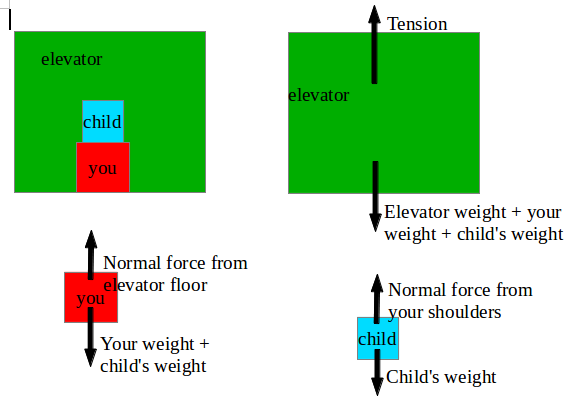
\includegraphics[scale=0.85]{figures/exam2problem2partA_image.png}
	\caption{elevator and two person system, and the forces acting on each person and the elevator.}
	\label{fig:partA}
\end{figure}

b. the tension is $11300$ Newtons
                                              
given the net acceleration $a_{net}$ and the masses of the elevator $m_{elev}$, you $m_{you}$, and
the child $m_{child}$, find the tension T using Newton's law.\newline
$(m_{elev} + m_{you} + m_{child})a_{net}$ = T - $(m_{elev} + m_{you} + m_{child})$g \newline
T = $(m_{elev} + m_{you} + m_{child})(g + a_{net})$ = $(1280.0 kg)(9.81 \frac{m}{s^{2}} - 1.00 \frac{m}{s^{2}})$\newline
T = $11276.8$ Newtons

c. weight force = $196$ Newtons downward   normal force = $176$ Newtons upward\newline
weight $m_{child}g = 196$ Newtons\newline
normal force from your shoulders $N_{child} = m_{child}(g + a_{net}) = (20.0 kg)(8.81 \frac{m}{s^{2}})$\newline
$N_{child} = 176$ Newtons

d. weight force = $765$ Newtons downward   normal force from floor = $705$ Newtons upward\newline
weight $m_{you}g + N_{child} = 765$ Newtons\newline
normal force from the floor $N_{floor} = (m_{you})(g + a_{net}) + N_{child} = (60.0 kg)(8.81 \frac{m}{s^{2}}) + 176$ Newtons
$N_{floor} = 705$ Newtons


%%%%%%%%%%%%%%%%%%%%%%%%%%%%%%%%%%%%%%%%%%%%%%%%%%%%%%%%%%%%%%%%%%%%%%%%%%%%%%%%
